\section{C2 EXTERNAL DATA REPRESENTATION, Presentation Layer} 
\rtext{Heterogeneity}
HW: Diff. HW architectures store bytes:Big, Small Endian
ProgrammingLanguage:Diff. PL store data types differently:AB, 0AB
\rtext{Transformation between representations}: Transformation between local and remote representations|Information may lost
\textbf{Two realizations}:
$1.$\textbf{Pairwise transformation between $n$ local representations}(vollständigGraph,$\#n^2 - n$, Either sender or receiver has to transform) 
$2.$\textbf{Transformation to and from canonical representation}(a single canonical $C$ as intermediate representation|No local information about communication
partner needed| $\#2*(n-2)$, $ -2$if canonical is one of $n$)
\rtext{XDR} encodes only data items, not information about their types
\textbar exactly 32 bit integer is stored according to \textbf{big endian} 
\textbar Data is encoded into blocks of multiples of 4: n-bytes contain data; r-bytes are used for padding with n + r mod 4 = 0
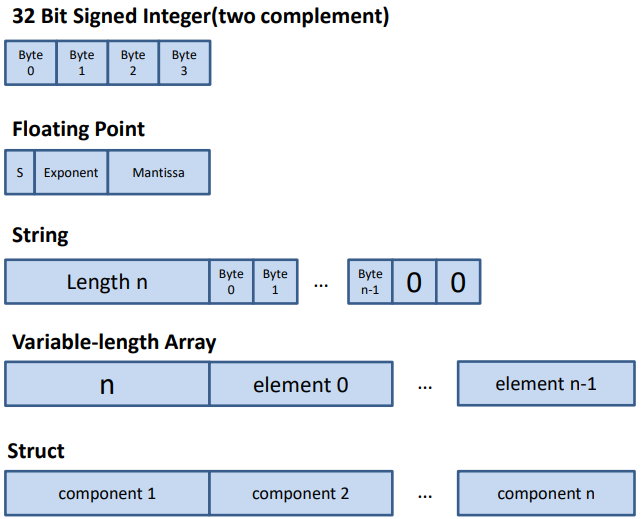
\includegraphics[width=.45\linewidth]{chap2_1.png} 
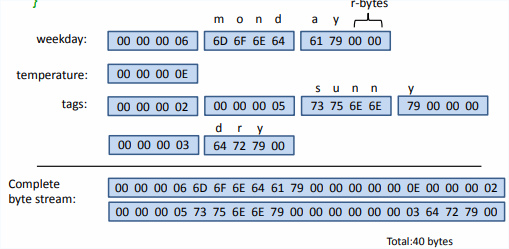
\includegraphics[width=.45\linewidth]{chap2_2.png} 
\lstinline{class file:String filename;int rights<>;String owner;}
\rtext{ASN.1}:Abstract description of data types \textbar Enables exchange in heterogeneous systems
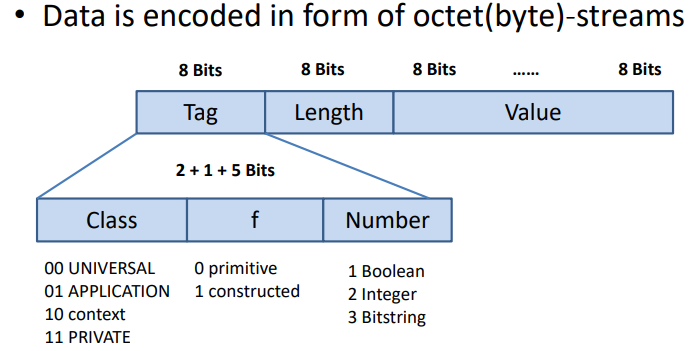
\includegraphics[width=.45\linewidth]{chap2_3.png}
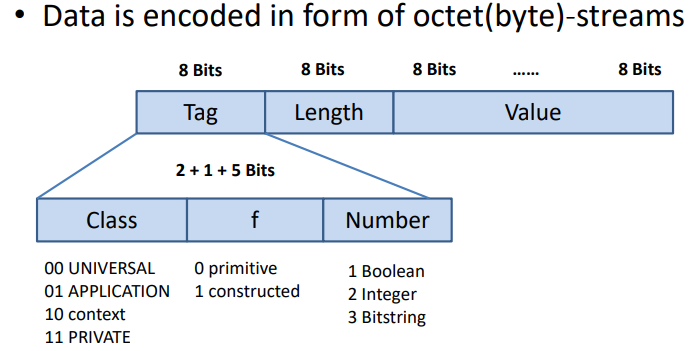
\includegraphics[width=.45\linewidth]{chap2_4.png}
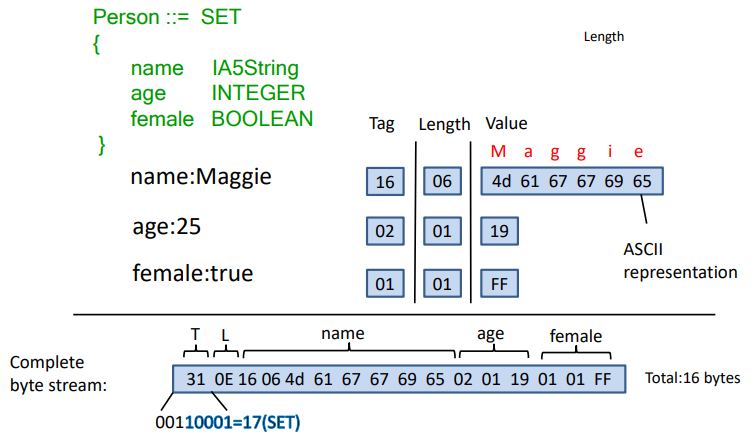
\includegraphics[width=.45\linewidth]{chap2_5.png}
\rtext{Java object serialization,JOS}
Stream-based transmission of serialized objects(Via TCP or UDP sockets)
, Receiver of object needs implementation of class
, Serialization does not require class specific code(Java reflection)
, Classes implements java.io.Serializable interface
\rtext{serialize:obj2bit}\lstinline{Socket s = new Socket("localhost", 8022);ObjectOutputStream oos = new ObjectOutputStream(s.getOutputStream()); oos.writeObject(obj);}
\rtext{deserialize:bit2obj}\lstinline{ServerSocket ss = new ServerSocket(8022);Socket s = serverSocket.accept();ObjectInputStream ois = new ObjectInputStream(s.getInputStream());obj=(Obj)ois.readObject();}